\section{Introduction} \label{introduction}
%% General Introduction
Machine learning techniques are increasingly being used in industrial and scientific applications to gain insight from the data.
Typically, a machine learning pipeline is a series of complex data processing steps to process a labeled training dataset and produce a machine learning model.
The machine learning model is then used to make predictions on new unlabeled data.
To fully utilize the model, it has to be deployed into an environment where it can answer prediction queries in real-time.

%% Intro to the problem of continuous improvement
After the model is deployed, new training data may become available.
In order to adapt to the new training data, one has to retrain and redeploy the model.
In many real-world use cases, training datasets are very large which may require hours of data processing and training to result in a new model.
Therefore, it is not feasible to train a new model frequently.
This means that the deployed model is not always up-to-date.
Online learning methods are utilized to provide fresh and up-to-date models.
However, unless the online learning method is highly tuned to the specific use case, they do not guarantee a high prediction accuracy \cite{ma2009identifying, macmahan2013}. 
This results in a trade-off between the model training cost and the model quality.
Moreover, any incoming prediction and training data has to be first processed by the same pipeline that was used during the initial training. 
Therefore, deploying models alone are not adequate and the entire pipeline has to be deployed as well.

%% Current Deployment Systems
Several existing platforms such as Velox, Clipper, TensorFlow Extended provide support for deployment of models with TensorFlow Extended being the only one that supports deployment of the entire machine learning pipeline \cite{crankshaw2014missing, crankshaw2016clipper, agarwal2014laser, baylor2017tfx}.
However, the existing systems only support online learning, periodical retraining, or a combination of the two for maintaining the quality of models.
In many cases, the amount of training data is very large, thus training a new pipeline may take hours (or even days) \cite{baylor2017tfx}.
During the retraining, incoming prediction requests are answered by the old model and new real-time training data are accumulated.
By the time the retraining is finished, enough data is accumulated to prompt for a new round of training.
As a result, in the current deployment platforms, the deployed models and pipelines are constantly out of date which results in lower prediction accuracy.

%% Use case
\begin{figure}[h!]
\centering
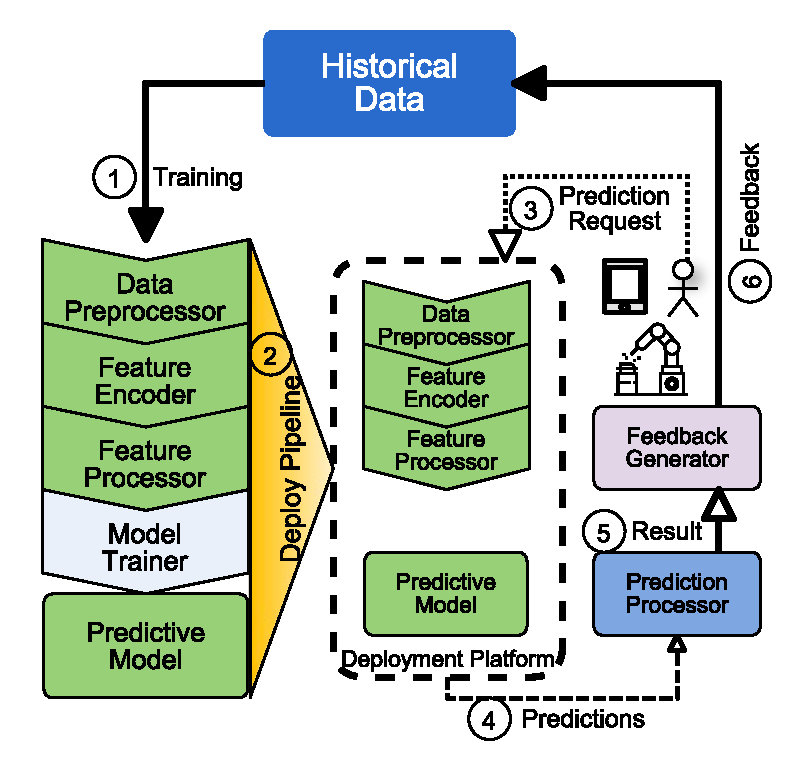
\includegraphics[width=\columnwidth]{../images/generic-motivational-example.pdf}
\caption{Deployment process of machine learning pipelines}
\label{fig:motivational-example}
\end{figure}

Figure \ref{fig:motivational-example} shows the typical deployment process of existing systems.
From an existing dataset, a pipeline consists of several data and feature processing steps, and a training algorithm is trained \textcircled{1}.
Then, a deployment platform deploys the model (with the pipeline) \textcircled{2} where the pipeline is used to process incoming prediction queries \textcircled{3} before the model makes a prediction  \textcircled{4}.
The resulting predictions are further processed and converted to meaningful actions before being presented back to the users or the entities issuing the prediction queries \textcircled{5}.
Based on the result of the prediction query, feedback, containing the original prediction query and the correct label, may be generated that is appended to the existing training data \textcircled{6}.
Throughout the deployment process, it is possible that the accuracy of the predictions being made drop below an acceptable threshold due to the changes in the distribution of the incoming prediction requests.
As a result, the model and the pipeline are regularly retrained and redeployed back into the deployment platform(\textcircled{1} to \textcircled{6} is repeated).

Several real-world use cases follow the workflow described in Figure \ref{fig:motivational-example}.
One example is the problem of Ad click prediction \cite{macmahan2013}.
In Ad click prediction, the machine learning pipeline typically consists of extracting features from the users and ads. 
Logistic regression models have shown to perform well in this setting \cite{macmahan2013}.
Prediction queries consist of the user's information and a pool of available ads for displaying to the user.
Once a prediction score for each of these ads are made, an Ads selector unit (similar to the Prediction Processor in Figure \ref{fig:motivational-example}) picks a set of ads with the highest score to display to the user.
Based on the action of the user (click or no click), new training data, containing the original prediction request and the label (+1 for a clicked ad and -1 for a non-clicked ads) will be generated which is stored with the existing training data (similar to the Feedback Generator in the Figure).
\hl{maybe another use case (IoT or Steel coil flatness prediction)}

The above example demonstrates the complexity of deployment and maintenance of machine learning pipelines through offline retraining.
A flexible deployment platform should, therefore, be able to meet the model quality requirement without requiring the periodical offline retraining of the models and pipelines.

%% Our solution
We propose a deployment platform that continuously updates the model (and the pipeline) using a combination of the historical and incoming data.
Our deployment platform updates the model using the incoming feedback data (we call this the real-time training data) similar to how online machine learning algorithms work while simultaneously performs small batch updates using the historical data.
Our solution offers two key optimizations.

\textit{Proactive training.}
Instead of fully training a new model using the historical training data, we continuously update the existing model using small sampled batches of the historical data.
The deployment platform first, forwards each batch of the data through the pipeline and then, performs a partial model update using the processed batch.
The updated model is immediately ready for answering prediction queries.
Our experiments show that proactive training of the model and pipeline achieves more accurate predictions over time and requires fewer resources when compared to the periodical retraining.

\textit{Online Statistics Computation and Feature Materialization}
Our deployment platform updates the model using the real-time training data by employing advanced online machine learning algorithms (such as Adagrad \cite{duchi2011adaptive}), before storing it for the proactive training.
Since the real-time training data is traveling through the pipeline during the online training phase, we compute statistics required by the pipeline stages, update the pipeline stages, and transform the data to the set of usable features required for the model before storing it with the rest of the historical data.
As a result, during the proactive training, the data and feature processing steps of the pipeline are skipped and the materialized features are directly used in the model trainer component of the pipeline.

% Our contributions
In summary, our contributions are:
\begin{itemize}
\item A platform for continuously training deployed machine learning models and pipelines that adapts to the changes in the incoming data.
\item Proactive training of the deployed models and pipelines that frequently updates the model in-place using a combination of the historical and the real-time data and increases the prediction accuracy when compared with state of the art.
\item Efficient pipeline processing and model training by online statistics computation and feature materialization, thus guaranteeing the availability of up-to-date models for answering prediction queries.
\end{itemize}

The rest of this paper is organized as follows:
Section \ref{continuous-training-serving} describes the details of our continuous training approach.
In Section \ref{sec:system-architecture}, we introduce the architecture of our deployment system.
In Section \ref{evaluation}, we evaluate the performance of our continuous deployment approach.
Section \ref {related-work} discusses the related work.
Finally, Section \ref{conclusion} presents our conclusion and the future work.
